\pdfoutput=1 % only if pdf/png/jpg images are used
\documentclass{JINST}

\usepackage{amsmath,amssymb}
\usepackage[numbers,sort]{natbib}
%\hypersetup{colorlinks, citecolor=blue, linkcolor=blue, filecolor=blue, urlcolor=red}

\title{Background rejection in NEXT using deep neural networks}

\author{NEXT Collaboration: Author 1$^a$\thanks{Corresponding author.},
Author 2$^b$\\
\llap{$^a$}Instituto de F\'isica Corpuscular (IFIC), CSIC \& Universitat de Val\`encia,\\ 
Calle Catedr\'atico Jos\'e Beltr\'an, 2, 46980 Paterna, Valencia, Spain\\
\llap{$^b$}University of Texas at Arlington\\
 701 S. Nedderman Drive, Arlington, TX 76019, USA\\
E-mail: \email{correspodingauthor@ific.uv.es}\\}

\bibliographystyle{unsrtnat}
%%%%%%%%%%%%%%%%%%%%%%%%%%%%%%%%%%%%%%%%%%%%%%%%%%
% $Id: commands.tex 1931 2015-01-17 10:32:50Z jmalbos $
% Some useful new commands...

%%%%%%%%%%%%%%%%%%%%%%%%%%%%%%%%%%%%%%%%%%%%%%%%%%
% BB
\newcommand{\bb}{\ensuremath{\beta\beta}}
% BB0NU
\newcommand{\bbonu}{\ensuremath{0\nu\beta\beta}}
% BB2NU
\newcommand{\bbtnu}{\ensuremath{2\nu\beta\beta}}

%%%%%%%%%%%%%%%%%%%%%%%%%%%%%%%%%%%%%%%%%%%%%%%%%%
% mBB
\newcommand{\mbb}{\ensuremath{m_{\bb}}}
% T0nu
\newcommand{\Tonu}{\ensuremath{T_{1/2}^{0\nu}}}
% Gonu
\newcommand{\Gonu}{\ensuremath{G^{0\nu}}}
% MNE
\newcommand{\Monu}{\ensuremath{\left|M^{0\nu}\right|}}
% Qbb
\newcommand{\Qbb}{\ensuremath{Q_{\bb}}}

%%%%%%%%%%%%%%%%%%%%%%%%%%%%%%%%%%%%%%%%%%%%%%%%%%
% kg·year
\newcommand{\kgy}{\ensuremath{\mathrm{kg}\cdot\mathrm{yr}}}
% Mbb
\newcommand{\Mbb}{\ensuremath{M_{\bb}}}
% kgbb
\newcommand{\kgbb}{\ensuremath{\mathrm{kg}_{\bb}}}
% ckky
\newcommand{\ckky}{\ensuremath{\mathrm{cts~keV^{-1}~kg^{-1}~yr^{-1}}}}
% ckkbby TO BE REVISED
\newcommand{\ckkbby}{\ckky}

%%%%%%%%%%%%%%%%%%%%%%%%%%%%%%%%%%%%%%%%%%%%%%%%%%
% Ca-48
\newcommand{\CA}{\ensuremath{^{48}\mathrm{Ca}}}
% Ge-76
\newcommand{\GE}{\ensuremath{^{76}\mathrm{Ge}}}
% Se-82
\newcommand{\SE}{\ensuremath{^{82}\mathrm{Se}}}
% Zr-96
\newcommand{\ZR}{\ensuremath{^{96}\mathrm{Zr}}}
% Mo-100
\newcommand{\MO}{\ensuremath{^{100}\mathrm{Mo}}}
% Pd-110
\newcommand{\PD}{\ensuremath{^{110}\mathrm{Pd}}}
% Cd-116
\newcommand{\CD}{\ensuremath{^{116}\mathrm{Cd}}}
% Sn-124
\newcommand{\SN}{\ensuremath{^{124}\mathrm{Sn}}}
% Te-130
\newcommand{\TE}{\ensuremath{^{130}\mathrm{Te}}}
% Xe-136
\newcommand{\XE}{\ensuremath{^{136}\mathrm{Xe}}}
% Nd-150
\newcommand{\ND}{\ensuremath{^{150}\mathrm{Nd}}}

% Ba-136
\newcommand{\BA}{\ensuremath{^{136}\mathrm{Ba}}}

% Tl-208
\newcommand{\TL}{\ensuremath{^{208}\mathrm{Tl}}}
% Bi-214
\newcommand{\BI}{\ensuremath{^{214}\mathrm{Bi}}}

\newcommand{\URANIUM}{Uranium}
\newcommand{\THORIUM}{Thorium}

% Xe-136
\newcommand{\NA}{\ensuremath{^{22}}Na}
\newcommand{\CS}{\ensuremath{^{137}}Cs}
\newcommand{\SEHF}{\ensuremath{\mathrm{SeF}_6}}
\newcommand{\COT}{\ensuremath{\mathrm{CO}_2}}
\newcommand{\CHF}{\ensuremath{\mathrm{CH}_4}}
\newcommand{\CFF}{\ensuremath{\mathrm{CF}_4}}



%%%%%%%%%%%%%%%%%%%%%%%%%%%%%%%%%%%%%%%%%%%%%%%%%%
% W-values
\newcommand{\Wi}{\ensuremath{W_\mathrm{i}}}
\newcommand{\Wsc}{\ensuremath{W_\mathrm{sc}}}




%%%%%%%%%%%%%%%%%%%%%%%%%%%%%%%%%%%%%%%%%%%%%%%%%%


\abstract{We investigate the potential of using deep learning techniques to reject background events in searches
for neutrinoless double-beta decay with high pressure xenon time projection chambers capable of detailed track
reconstruction.  The differences in the topological signatures of background and signal events can be learned
by deep neural networks via training over many thousands of events.  These networks can then be used to classify
further events as signal or background, providing an additional background rejection factor at an acceptable loss of
efficiency.  This method is found to perform substantially better than previous methods developed based on the use of the
same topological signatures and has the potential for further improvement.}

\keywords{Neutrinoless double beta decay; deep neural networks; TPC; high-pressure xenon chambers;  Xenon; NEXT-100 experiment}

\begin{document}

\section{Introduction}\label{sec:intro}
\noindent Neutrinoless double-beta decay (\bbonu) is a rare nuclear process in which the nuclear charge changes by two units, and the full energy of the decay ($Q_{\beta\beta}$) is 
emitted in the form of two electrons (or positrons).  It is essentially two simultaneous $\beta^{+}$ or $\beta^{-}$ decays in which no neutrinos are emitted.  While two-neutrino double-beta 
decay ($2\nu\beta\beta$), two simultaneous beta decays in which the two neutrinos are present, is a process predicted by the standard model that has been observed in several isotopes, 
\bbonu\,has never been observed, even after over 75 years of experimental effort.  If \bbonu\,does exist, this implies that the neutrino is its own anti-particle, that is, a
a Majorana particle \cite{Schechter_1982}, amongst other important physical implications (see for example \cite{GomezCadenas:2013ue, Cadenas_2012, Avignone_2008}).

The detection of \bbonu\,decay continues to present unique experimental challenges.  For a given isotope, the lifetime of \bbonu\,decay depends on a nuclear matrix element, 
which can be calculated to some uncertainty, and the square of the effective neutrino mass $|m_{\beta\beta}|^2 = |\sum_{i=e,\nu,\tau}U_{ei}^2m_{i}|^2$ which is a combination of the neutrino
masses $m_{i}$ and neutrino mixing matrix elements $U_{ei}$.  The lifetime is relatively shorter for a degenerate neutrino mass hierarchy ($m_1 \sim m_2 \sim m_3$), longer for an inverted 
neutrino mass hierarchy ($m_1 \ll m_2 < m_3$), and longest for a normal mass hierarchy ($m_1 < m_2 \ll m_3$).  Experiments of the current generation contain approximately
100 kg of the candidate isotope and are subject to several tens of counts per year of background events in their region of interest of energy selection near $Q_{\beta\beta}$.  These experiments
will be capable of probing only the parameter space corresponding to the degenerate mass hierarchy, perhaps pushing into the inverted hierarchy.  In order to completely cover the parameter 
space of the inverted mass hierarchy, experiments employing candidate isotope masses at the ton-scale with background rates of several counts per ton-year will be required.  

NEXT (Neutrino Experiment with a Xenon TPC) \cite{Gomez-Cadenas:2014dxa} will search for neutrinoless double-beta decay in the Lab using a Time Projection Chamber (TPC) filled with 100 kg of 
high-pressure xenon gas (HPXe) at 15 bar pressure enriched to 90\% in the candidate isotope $^{136}$Xe.  The detector will operate using electroluminescent readout (see figure \ref{fig.SS}), in which 
ionization electrons are drifted in a region of relatively low electric field to a narrow region of relatively high electric field, in which they are then accelerated to energies high enough to excite but not 
ionize the atoms of the xenon gas.  These excitations give rise to the emission of electroluminescent light which is detected by an energy plane of 60 photomulitplier tubes (PMTs) and a tracking 
plane of about 8000 silicon photomultipliers (SiPMs).  The detected electroluminescent light signal is called (S2), and can be compared in time with the light detected (S1) due to the excitations 
produced during the initial creation of the ionization track to determine the z-coordinate of its production.  The pattern of light observed on the tracking plane, located just behind the narrow 
electroluminescent region, can be used to obtain the x-y location of the ionization electrons producing the corresponding S2.  The result is a 3D image of the ionization track produced within the 
detector.  The amount of S2 light detected by the energy plane gives an accurate measurement of the energy of the event.  Together this information can be used to identify potential 
\bbonu\,events from the various energy depositions produced in the active volume.

\begin{figure}[!htb]
	\centering
	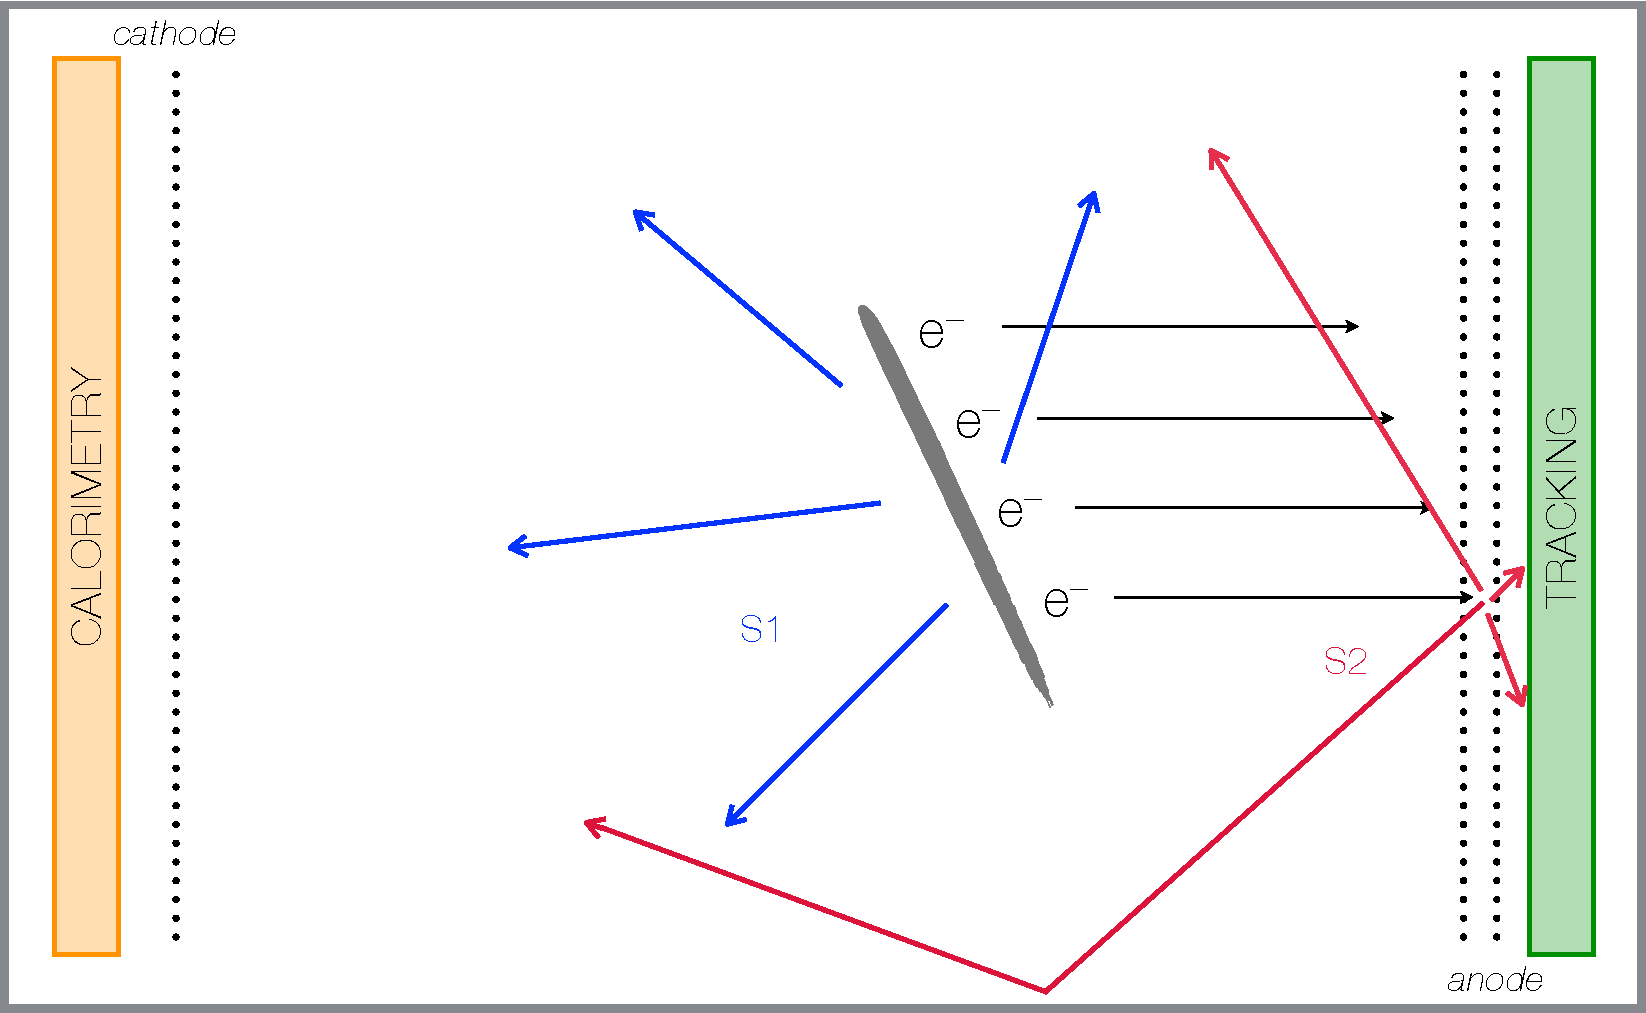
\includegraphics[width= 0.95\textwidth]{fig/SoftAsymmetric_bound.pdf}
	\caption{Production and detection of S1 and S2 in an asymmetric HPXe TPC (figure from \cite{MartinAlbo_thesis}).} \label{fig.SS}
\end{figure}

In addition to performing a competitive search for \bbonu, NEXT will demonstrate potential 
techniques for operation and background rejection at the ton-scale.  The NEXT collaboration has already built and tested several kg-scale prototypes, NEXT-DBDM \cite{Alvarez:2012kua} and
NEXT-DEMO \cite{Alvarez:2012xda,Alvarez:2012kua,Alvarez:2013gxa,Lorca:2014sra}, which have both demonstrated the excellent energy resolution (extrapolated to 0.5-0.7\% FWHM at
$Q_{\beta\beta}$) obtainable in high pressure xenon gas.  NEXT-DEMO has demonstrated the feasibility of signal/background discrimination based on the topology of reconstructed tracks,
an essential component to identifying \bbonu\,events and rejecting background events (see section \ref{sec:topology}).  The collaboration is currently constructing the first phase of the experiment NEXT-NEW, a 10 kg prototype 
containing about 20\% of the sensors of the 100 kg detector (NEXT-100).  By confirming the ability to obtain good energy resolution and reconstructed tracks at several different scales, NEXT 
intends to confirm the suitability of high pressure xenon gas for operation at the ton-scale.

\section{The NEXT Topological Signature}\label{sec:topology}
One of the most important aspects of NEXT is its ability to image the ionization tracks produced by energetic electrons in its active volume.  Double-beta decay events have a distinct
topological signature produced by two electrons emitted from a common vertex.  Such a track is substantially different from that of a single electron produced, for example, by photoelectric
conversion of a high-energy gamma ray due to several factors.  First, the ionization density ($dE/dx$) increases rapidly with decreasing energy as the energy of the electron drops below about 1 MeV.  Furthermore, electron multiple scattering, the repeated scattering of the electron throughout the creation of its ionization path, also becomes more intense at lower energies.  Together
these effects lead to a single-electron track that is long and relatively smoother near its beginning and becomes increasingly contorted until the electron comes to a stop, depositing
its final several hundred keV of energy in a relatively smaller volume, which we describe as a ``blob.''  A double-beta event will look like two such tracks beginning at a single vertex.  Figure \ref{fig.ETRK2} compares the two types of
tracks.  Our goal is to identify signal events and reject background events by analyzing the topology of the reconstructed track.  Here we will discuss how this is done by reconstructing an ordered
track, locating the endpoints, and determining whether.  Later we will investigate the performance of deep learning techniques which should address, in principle, all details of the topology 
of the entire track.

\begin{figure}[!htb]
	\centering
	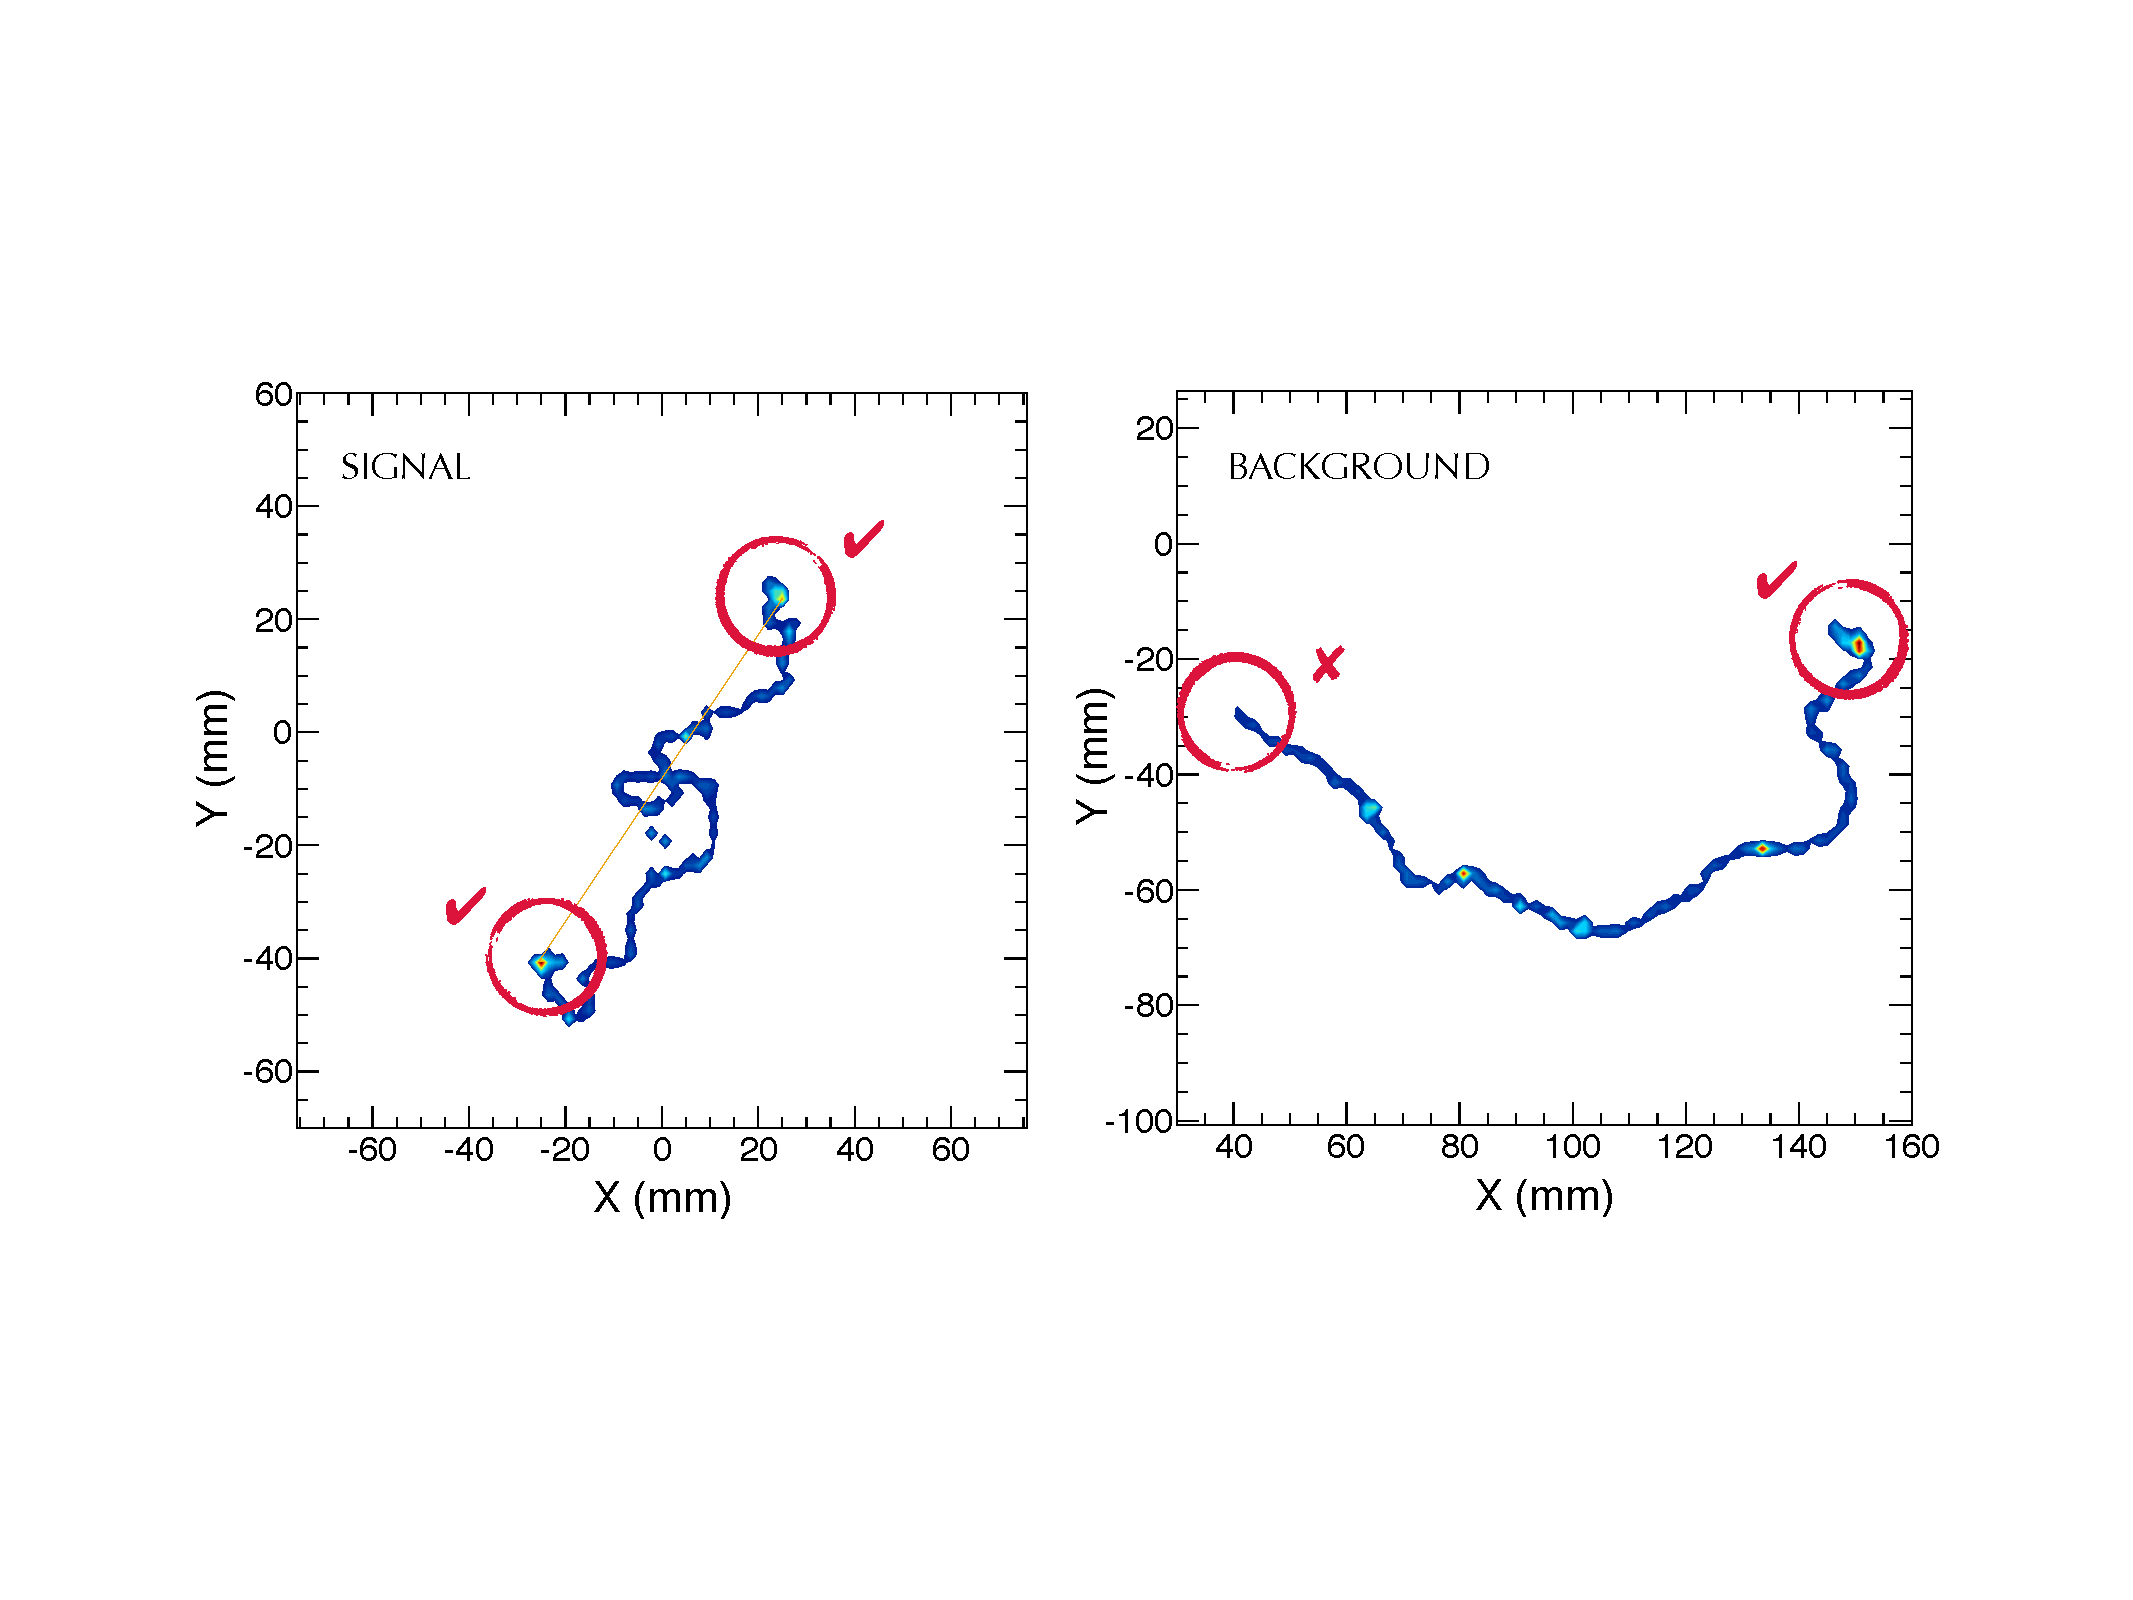
\includegraphics[width= 0.95\textwidth]{fig/TrackSignature.pdf}
	\caption{Monte Carlo simulated \bbonu\,(left) and background (right) events.  The simulation was done in xenon gas at a pressure of 15~bar. Signal events consist of two electrons emanating
		from a common vertex, producing two initially smooth tracks ending in two dense energy depositions (or ``blobs'').  Background events consist of one long track terminating in one
		single ``blob'' (figure from \cite{MartinAlbo_thesis}).} \label{fig.ETRK2}
\end{figure}

\subsection{Monte Carlo Simulation}\label{ssec:NEXT100MC}
The central Monte Carlo simulation in this study was performed in GEANT4 \cite{GEANT4}, and the full geometry of the NEXT-100 detector was modeled.  \bbonu\,events were
simulated randomly throughout the active region, and gamma rays of energies 2.447 MeV and 2.614 MeV (corresponding to gammas emitted by daughters of $^{214}$Bi and $^{208}$Tl,
respectively, two naturally occurring radioactive isotopes) were launched in the Monte Carlo from several different regions within the detector geometry. % confirm these energies with Javi 
The resulting locations and magnitudes of the energy depositions in the active volume were recorded by GEANT4 as hits with a 1 mm minimum step size, and each event was then
analyzed according to the following procedure:

\begin{enumerate}
	\item[1.] A fiducial cut was applied to the true Monte Carlo hits, ensuring that no more than 10 keV of energy was deposited within 2 cm of the edges of the active region.
	\item[2.] An energy cut was applied to the true Monte Carlo energy, ensuring that all events contained a total deposited energy between 2.3 and 3.0 MeV.
	\item[3.] The total energy of each event was smeared according to a detector resolution of 0.7\% FWHM.
	\item[4.] An energy cut was appied ensuring a smeared energy of between 2.3 and 2.4 MeV.
	\item[5.] The set consisting of true Monte Carlo hits was converted into one or more subsets of connected voxels.  A voxel was defined to be a small cubical volume of a chosen 
	length, width, and height.  3D space was divided into voxels of the specified size, and the (smeared) energy of each hit was placed in the voxel in which it was located according to its
	true position.  A connected set of voxels, one in which each voxel neighbored at least one other voxel in the set, was called a track, where ``neighboring'' voxels shared at least one face, edge,
	or corner.
	\item[6.] A cut was made passing only events with exactly one single track.  This was done to simplify further analysis and could in principle be relaxed in the future.
\end{enumerate}

At this point, the events were deemed to be ready to be analyzed according to their topological signature.  Note that the single track cut alone eliminated a significantly larger number of 
background events than signal events, as the background events originated from gammas which had a higher probability of being subject to physics yielding a multi-site track (e.g., Compton 
scattering).

\subsection{Topological Analysis}\label{ssec:TopologicalAnalysis}
After being subject to the cuts described in the previous section, the events were classified as signal or background based on the presence of one or two ``blobs'' of energy in the
reconstructed track.  The procedure followed was similar to the one described in \cite{NEXT_topology}.  The track was reconstructed by finding the shortest path between each two 
pairs of connected voxels (using the Breadth First Search (BFS) algorithm), and choosing the longest of these paths to be the ordered path.  Note that such a path may not have included, 
in fact most likely did not include, all voxels in the event.  The first and last voxels in the path
were considered to be the beginning and end of the track.  The energy in all voxels that were located within a given radius $r_b$ of the beginning of the track was summed to give
an energy $E_{b,1}$, and similarly at the end of the track to give an energy $E_{b,2}$.  The histogram of $E_{b,1}$ vs. $E_{b,2}$ is shown in figure \ref{fig.blobcuts} for both signal and
background events.  In this case, the distance between a voxel and the extremes of the track was calculated as 
``along-the-track distance,'' in which the distance between any two voxels was integrated along the reconstructed track (as opposed to computing the Euclidean distance).  (How are voxels
not in the main track treated?)

\begin{figure}[!htb]
	\centering
	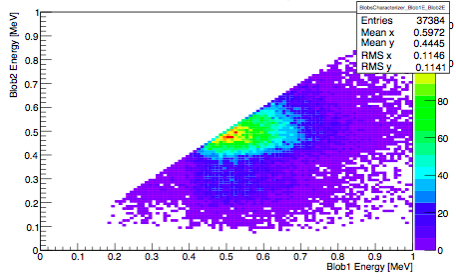
\includegraphics[scale = 0.45]{fig/blobcuts_bb0nu_2x2x2_E1vsE2.png}
	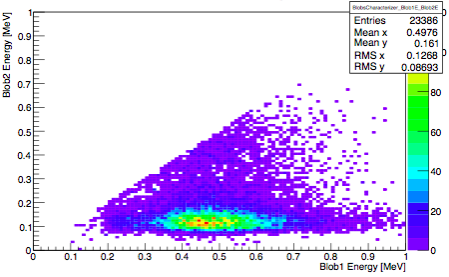
\includegraphics[scale = 0.45]{fig/blobcuts_Tl208_2x2x2_E1vsE2.png}
	\caption{Computed blob energies $E_{b,1}$ vs. $E_{b,2}$ for $r_b = 15$ mm for signal (left) and background ($^{208}$Tl right) events.} \label{fig.blobcuts}
\end{figure}

Now by applying a cut selecting signal events with two blobs, mandating that $E_{b,1} > 0.3$ MeV and $E_{b,2} > 0.3$ MeV, we eliminate all but 8.79\% of background ($^{208}$Tl) events 
and keep 84.15\% of signal events.  The same procedure rejected all but 7.80\% of background events due to $^{214}$Bi.

\section{Deep Learning}
The use of artificial neural networks to solve problems has been explored since the 1940s.  In recent years, with the dramatic increase in available computing power, the use of computationally
intense neural networks with many inner layers has become feasible.  These neural nets that are many layers deep, called deep neural networks (DNNs), are capable of learning large
amounts of data exhitibing a vast array of features.  This idea of ``deep learning'' has been applied to yield outstanding performance in solving difficult problems such as image and 
speech recognition.

% Details of GoogLeNet
In this study ... (describe the details of convolutional layers and GoogLeNet)

\section{Event classification with a DNN}
Here we investigate the performance of a DNN in classifying events into two categories, ``signal'' and ``background,'' and compare the results to the conventional analysis described in
section \ref{ssec:TopologicalAnalysis}.  We chose to use the GoogLeNet \cite{Googlenet} DNN for this initial study, as its implementation was readily available in the Caffe \cite{jia2014caffe}
deep learning framework along with an interface, DIGITS \cite{DIGITS}, which allows for fast creation of image datasets and facilitates their input to several DNN models.  For each simulated
dataset, GoogLeNet was trained on several tens of thousands of input events on a single GPU (either a GeForce GTX TITAN or GeForce GTX TITAN X, depending on the dataset), and several
thousand additional events as validation.  Each event was input to the net as a .png image consisting of three
color (RGB) channels, one for each of three projections of the 3D voxelized track, (R, G, B) $\rightarrow$ (xy, yz, xz).  This information for a signal event and a background event is
shown in figure \ref{fig.exampleProjs}.

\begin{figure}[!htb]
	\centering
	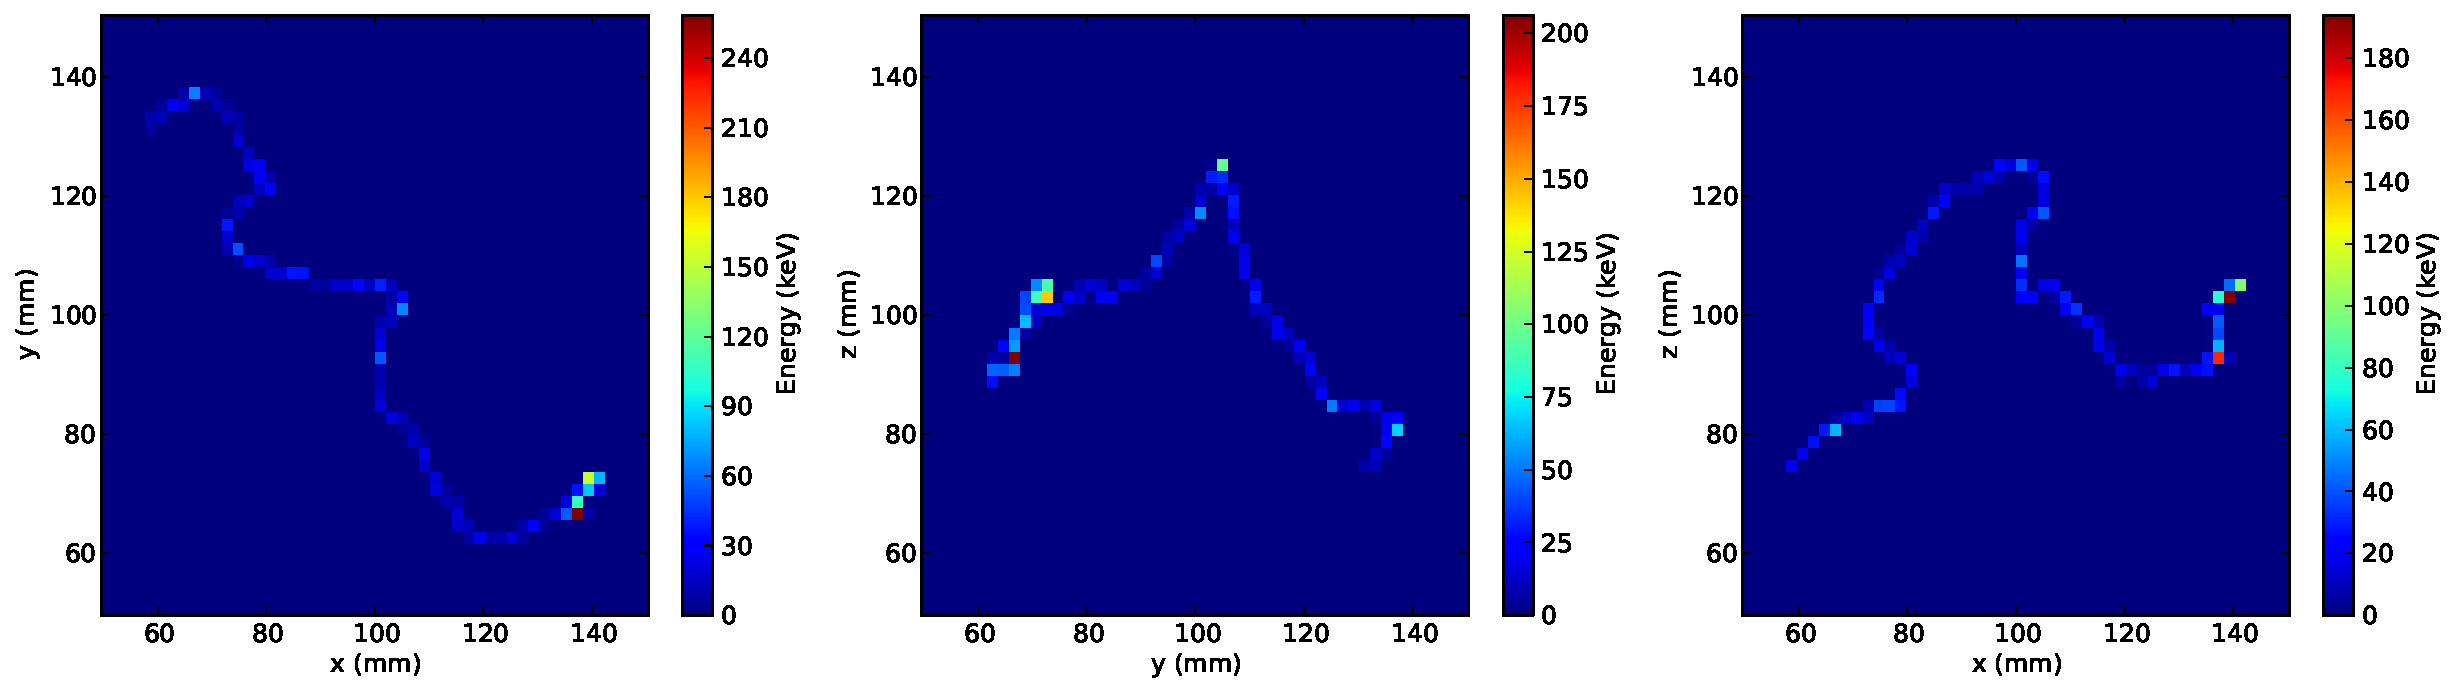
\includegraphics[scale=0.36]{fig/plt_h2D_vox_dnn3d_NEXT100_Paolina222_v2x2x2_r200x200x200_0_bg.pdf}
	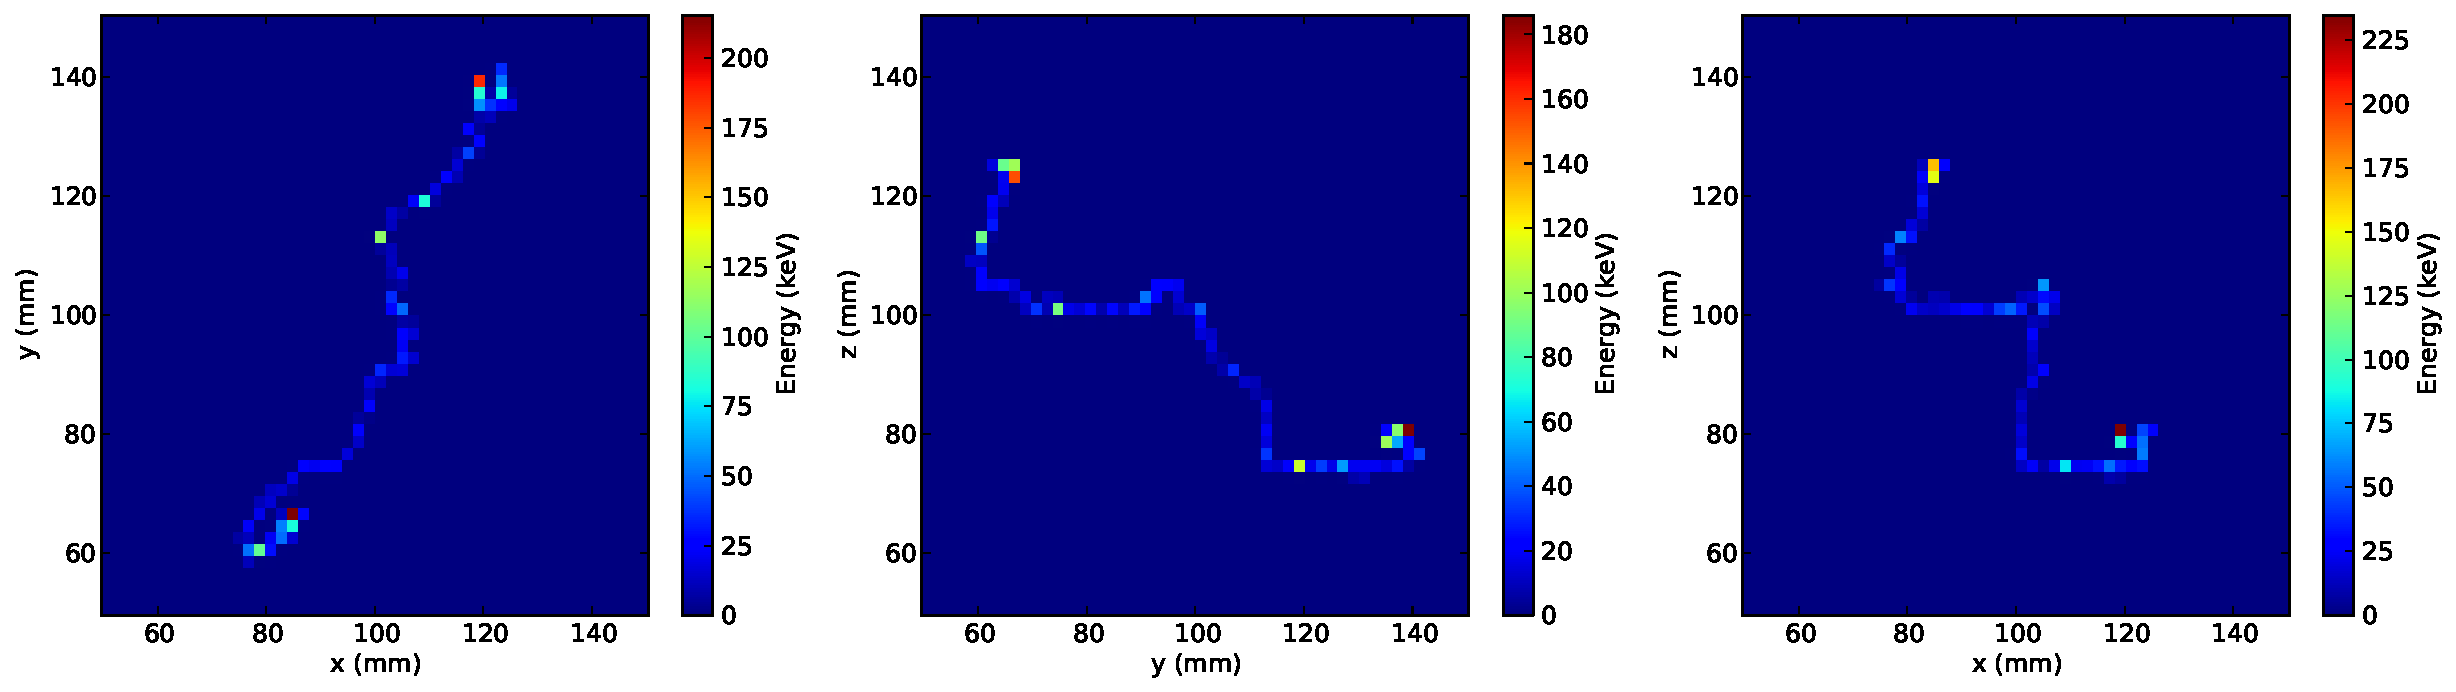
\includegraphics[scale=0.36]{fig/plt_h2D_vox_dnn3d_NEXT100_Paolina222_v2x2x2_r200x200x200_2_si.pdf}
	\caption{\label{fig.exampleProjs}Projections in xy, yz, and xz for an example background (above) and signal (below) event.}
\end{figure}

\subsection{Analysis of NEXT-100 Monte Carlo}\label{ssec:NEXTMCanalysis}
To compare the ability of the DNN to classify events directly with the performance of the topological analysis of section \ref{ssec:TopologicalAnalysis}, we consider NEXT-100 Monte Carlo 
events that have passed all cuts (1-6) described in section \ref{ssec:NEXT100MC}.  The GoogLeNet DNN was trained on 30000 such events (15000 signal and 15000 background) over 30 epochs, 
and an independent set of 12000 (6000 signal and 6000 background) events was used as a test dataset.  Because these were the exact same events as those used in the previous
topological analysis, the classification into signal and background from both analyses can be compared directly.  The results are shown in table \ref{tbl.DNNcomparison}.  The DNN
analysis performs better than the conventional analysis, but there is still potential room for improvement.  
	
\begin{table}[!htb]
	\begin{center}
		\caption[DNN analysis summary]{\label{tbl.DNNcomparison}Comparison of conventional and DNN-based analyses.  The comparison shows, for a given percentage of signal events
			correctly classified, the number of background events accepted (mistakenly classified as signal).}
		\begin{tabular}{ccc}
			\\
			\textbf{Analysis} & \textbf{Signal efficiency (\%)} & \textbf{Background accepted (\%)}\\
			\hline
			DNN analysis & 84.16 & 5.00\\
			Conventional analysis & 84.15 & 8.79\\
		\end{tabular}
	\end{center}
\end{table}

Because the output layer of the DNN gives a probability that a given event is signal and a probability that it is background, and these probabilities add to 1, a threshold may be 
chosen for determining whether an event is classified as signal or background.  It can be simply chosen as 50\%, meaning the category with greatest probability is the classification of the
event, or it can be varied to reject further background at the expense of signal efficiency.  Figure \ref{fig_svsb} shows the corresponding pairs of signal efficiency and background 
rejection produced by variation of this threshold, while for the values reported in table \ref{tbl.DNNcomparison} the threshold was chosen such that the signal efficiency matched that reported in 
the conventional analysis.

\begin{figure}[!htb]
	\centering
	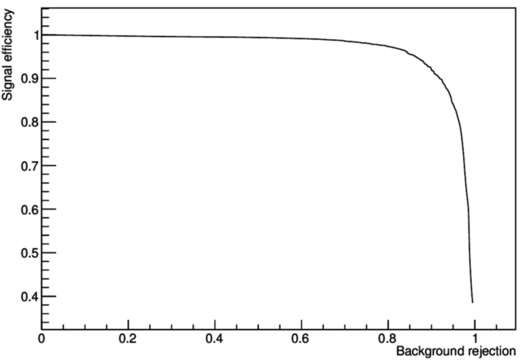
\includegraphics[scale=0.48]{fig/sigvsb_2x2x2_DNN.png}
	\caption{\label{fig_svsb}Signal efficiency vs. background rejection for DNN analysis of voxelized (2x2x2 cubic mm), single-track NEXT-100 Monte Carlo events.}
\end{figure}

\subsection{Evaluating the DNN analysis}\label{ssec:DNNeval}
We now ask what is causing some significant fraction of the events to be misclassified in the analysis described in section \ref{ssec:NEXTMCanalysis}.  A similar analysis was run on 
several different Monte Carlo datasets generated with differing physics effects with the hopes of better understanding where potential improvements could be made.

A simple Monte Carlo, which we call the ``toy Monte Carlo'' or ``toy MC,'' was designed to produce ionization tracks of single-electron and two-electron events with a fixed energy
considering minimal physical effects.  Discrete energy depositions were produced with a step size less than 1 mm according to the average stopping power $dE/dx$ as tabulated by
NIST \cite{NIST_mac} for xenon at 15 atm.  Electron multiple scattering was modeled by casting random gaussian numbers to determine the angles $\theta_{x}$ and $\theta_{y}$ of deflection, 
assuming the particle's direction of travel is $\hat{\mathbf{z}}$, and the angles $\theta_{x}$ and $\theta_{y}$ are the angles between the scattered direction and $\hat{\mathbf{z}}$ projected on 
the x-z and y-z planes respectively, as

\begin{equation}\label{eqn_mscat}
\sigma^{2}(\theta_{x,y}) = \frac{13.6\,\,\mathrm{MeV}}{\beta p}\sqrt{dz/L_{0}}\bigl[1 + 0.038\ln(dz/L_{0})\bigr].
\end{equation}

\noindent where $dz$ is the thickness of xenon travelled in this step, $L_{0}$ is the radiation length in xenon, $p$ is the electron momentum in MeV/c, and $\beta = v/c$, assuming $c = 1$.

Such tracks were generated and voxelized similar to the procedure described in point 5 of section \ref{ssec:NEXT100MC}.  Note that no ``single-track'' cut was necessary because no
physics generating a secondary track was implemented.  Also no energy smearing was performed.  For background events, the track generation began with a single electron emitted in a
random direction with energy 2.4578 MeV, while for signal events, this energy was shared equally between two electrons emitted in random directions from a single initial vertex.  The DNN
classified the resulting events with nearly 100\% accuracy.  Several modifications were then made to attempt to gain insight into the physics causing the lower classification observed in the
more detailed Monte Carlo tracks.  First, a realistic distribution of energies of the two electrons in signal events \cite{Ponkratenko_2000} was used, and later the magnitude of the multiple scattering was doubled (the prefactor 13.6 in equation \ref{eqn_mscat} was increased to 27.2).  The electron energy distribution caused a loss of about 1\% in average accuracy, and the
increased multiple scattering an additional 1\%.  However, even the two effects together were not enough to account for the inaccuracy of about 7\% observed in the events produced by the
full Monte Carlo.

Therefore an alternate GEANT-based Monte Carlo was run in which the detector geometry was not present, and background events (single electrons) and signal events (two electrons emitted
from a common vertex with a realistic \bbonu\,energy distribution) were generated in a large box of pure xenon gas at 15 bar.  An insignificant amount of energy smearing was applied to these
events, and they were then subject to the same voxelization procedure and single-track cut as described in section \ref{ssec:NEXTMCanalysis} point 5.  Under these controlled conditions, many 
events could be generated with different aspects of the physics switched on/off.  It was confirmed that with the same physics as that used in the NEXT-100 Monte Carlo, the DNN classified events 
with similar accuracy as before.  Disabling bremsstrahlung seemed to have little effect on the accuracy.  Disabling energy fluctuations in GEANT had some small effect (approx. 1\% increase in
accuracy), and disabling the production of secondaries (disallowing the production of secondaries with a range of less than 20 cm) had a more sigificant effect (approx. 2.5\% increase in accuracy),
though still did not yield accuracy similar to the toy MC datasets.  It was found that disabling both energy fluctuations and the production of secondaries gave accuracies similar to the toy MC
(about 98\%), and therefore we can conclude these are the physical effects that are often deceiving the DNN.

A summary of the Monte Carlo simulations run and the classification accuracies obtained is given in table \ref{tbl.DNNsummary}.  

\begin{table}[!htb]
	\begin{center}
		\caption[DNN analysis summary]{\label{tbl.DNNsummary}Summary of DNN analysis for different Monte Carlo datasets.  The accuracy was computed assuming that the classification
			of the DNN corresponded to the category (signal or background) with the higher ($> 50$\%) probability.  In each case, approximately 15000 signal and 15000 background events were
			used in the training procedure, and between 2000-3000 signal and 2000-3000 background events independent of the training set were used to determine the accuracy.}
		\begin{tabular}{rc}
			\\
			\textbf{Run description} & \textbf{Average accuracy} (\%)\\
			\hline
			toy MC, ideal & 99.8\\
			toy MC, realistic \bbonu\,distribution & 98.9\\
			Xe box GEANT4, no secondaries, no E-fluctuations & 98.3\\
			Xe box GEANT4, no secondaries, no E-fluctuations, no bremsstrahlung & 98.3\\
			toy MC, realistic \bbonu\,distribution, double multiple scattering & 97.8\\
			Xe box GEANT4, no secondaries & 94.6\\
			NEXT-100 GEANT4 & 93.1\\
			Xe box GEANT4, no E-fluctuations & 93.0\\
			Xe box, no bremsstrahlung & 92.4\\
			Xe box, all physics & 92.1
		\end{tabular}
	\end{center}
\end{table}

The production of a large secondary (``delta'') electron near the beginning of the track in a single-electron event, for example, could produce an event that looks almost indistinguishable from 
a double-beta event in topology.  (Discuss further the ``zoology'' of events misclassified by the DNN.)

\section{Conclusions}
DNN analysis with just three projections seems to be capable of outperforming conventional analysis.  Discuss future plans to develop an optimized DNN analysis and speculate
on possible improvements.

\acknowledgments

This work was supported by the European Research Council under the Advanced Grant 339787-NEXT and the Ministerio de Econom\'{i}a y Competitividad of Spain under Grants CONSOLIDER-Ingenio 2010 CSD2008-0037 (CUP), FPA2009-13697-C04-04, FPA2009-13697-C04-01, FIS2012-37947-C04-01, FIS2012-37947-C04-02, FIS2012-37947-C04-03, and FIS2012-37947-C04-04.  JR acknowledges support from a Fulbright Junior Research Award.

\bibliography{dnnext}


\end{document}